\begin{figure}[H]
    \centering
    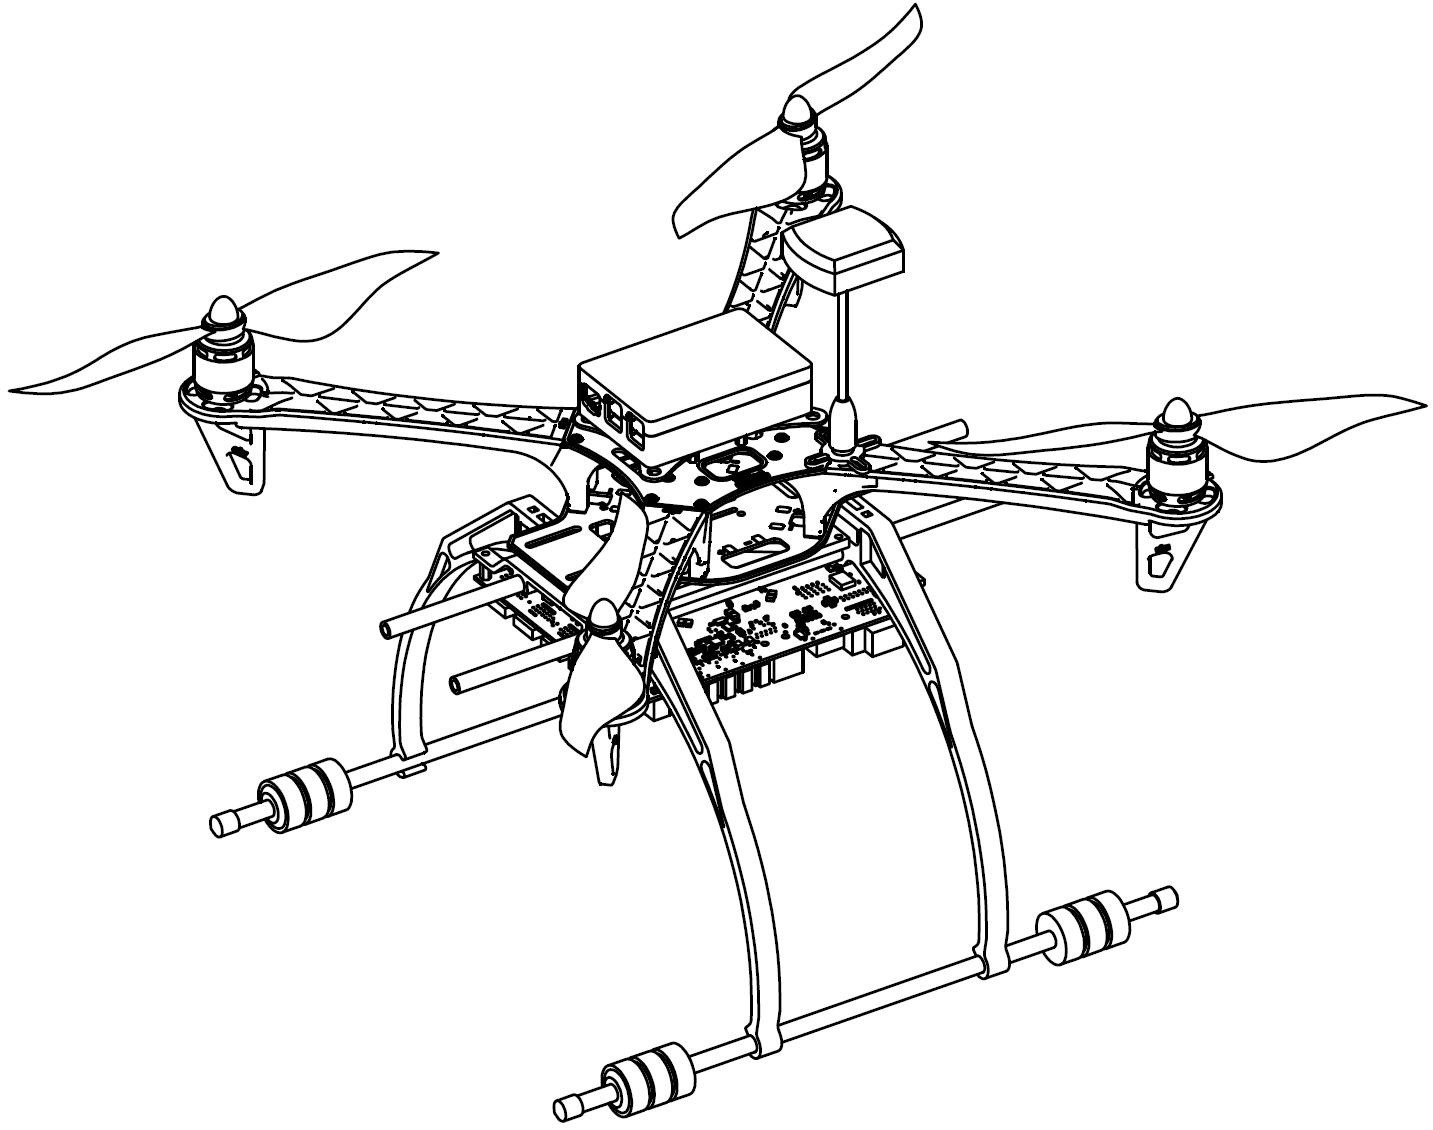
\includegraphics[width=0.85\textwidth]{img/testrigcad1.png}
    \caption{Team 109 Testing Rig Prototype using RPAS Generously Provided by Yiyi Yan and UBC \textit{Unmanned Aerial Systems}}
    \label{fig:testrigcad1}
\end{figure}

The bare-minimum multirotor remote-piloted aerial system (RPAS) or informally referred as ``drone'', consists of a propulsion system, flight controller, speed controllers, battery, and sensor systems. Our testing rig is shown  in Figure~\ref{fig:testrigcad1}

\subsubsection{Multirotor Configuration}

A multirotor RPAS (MRPAS) has several common configurations: a tricopter, a quadcopter, and a hexacopter (as seen in Figure~\ref{fig:rpas-config}).

\begin{figure}[b]
    \centering
    \begin{subfigure}[b]{0.3\textwidth}
        \centering
        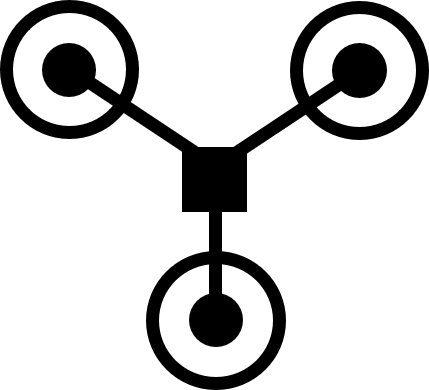
\includegraphics[scale=0.4]{img/drone_yconfig}
        \caption{Tricopter Y-Configuration}
        \label{fig:tricopter-y}
    \end{subfigure}
    ~
    \begin{subfigure}[b]{0.3\textwidth}
        \centering
        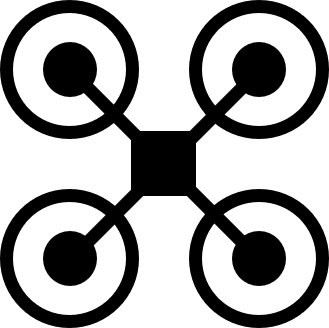
\includegraphics[scale=0.4]{img/drone_xconfig}
        \caption{Quadcopter X-Configuration}
        \label{fig:quadcopter-x}
    \end{subfigure}
    ~
    \begin{subfigure}[b]{0.3\textwidth}
        \centering
        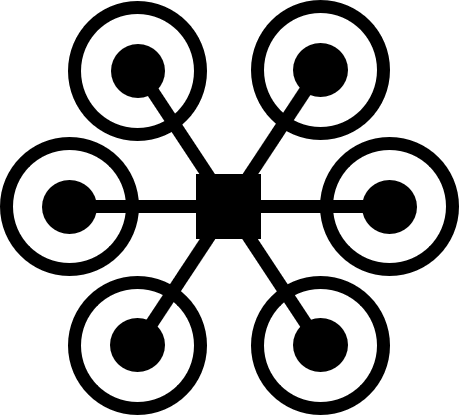
\includegraphics[scale=0.4]{img/drone_hexconfig}
        \caption{Hexcopter X-Configuration}
        \label{fig:hexcopter-x}
    \end{subfigure}
    
    \caption{Multirotor RPAS Configurations}
    \label{fig:rpas-config}
\end{figure}

\textbf{Tricopter:} Tricopters requires fewer motors and speed controllers, implying less components and power draw required to sustain flight. The angle between each motor arm is also wider at 120 degrees and thus reduces obstruction from camera views. 

\begin{figure}[h]
    \centering
    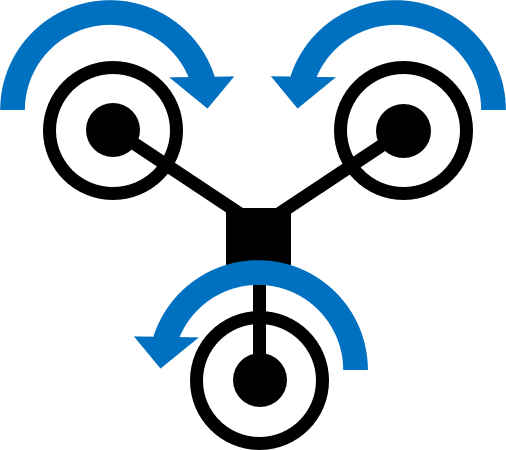
\includegraphics[scale=0.4]{img/drone_yconfigt}
    \caption{Tricopter Y-configuration}
    \label{fig:tricopter-y-t}
\end{figure}

However, systems with an odd-number of actuators are inherently unstable due to the asymmetry of the motor torque as shown in Figure~\ref{fig:tricopter-y-t}. Therefore, this design requires an additional servo motor (consists of a DC motor and a gear box) to precisely control the tail motor angle of tilt to counter the excess torque --- similar to the tail of a helicopter.

This configuration is not suitable for our application since it requires increased control complexity. The compromise is not worth the agility that this configuration provides, and we rather place more emphasis on flight stability.

\textbf{Quadcopter X:}
The quadcopter is the most common configuration in consumer multirotor products. The quadcopter is more stable than a tricopter as it utilizes four motors, as seen in Figure \ref{fig:quadcopter-x-t}. Two of the motors spin clockwise and the other two spin counter-clockwise --- effectively cancelling each other’s undesired torque. Applying the same power into each motor allows the MRPAS to hover in place. We can perform 6 degree-of-freedom (DOF) movements by applying a combination of differential thrusts to each motor (Figure \ref{fig:rpas_6dof}).

\begin{figure}[h]
    \centering
    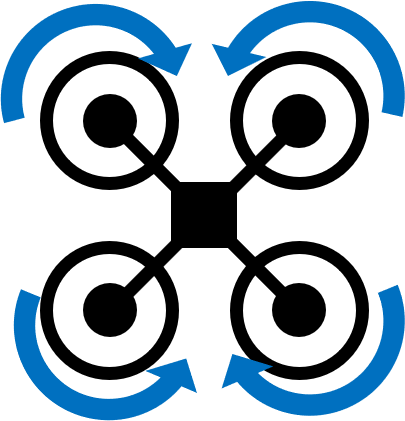
\includegraphics[scale=0.4]{img/drone_xconfigt}
    \caption{Quadcopter X-configuration}
    \label{fig:quadcopter-x-t}
\end{figure}

\begin{figure}[h]
    \centering
    \begin{subfigure}[b]{0.3\textwidth}
        \centering
        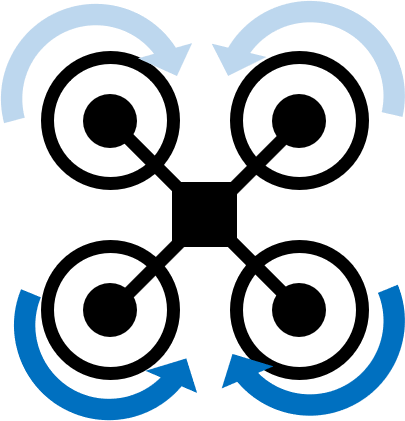
\includegraphics[scale=0.4]{img/drone_x_pitch}
        \caption{Pitch forward}
        \label{fig:x-pitch}
    \end{subfigure}
    ~
    \begin{subfigure}[b]{0.3\textwidth}
        \centering
        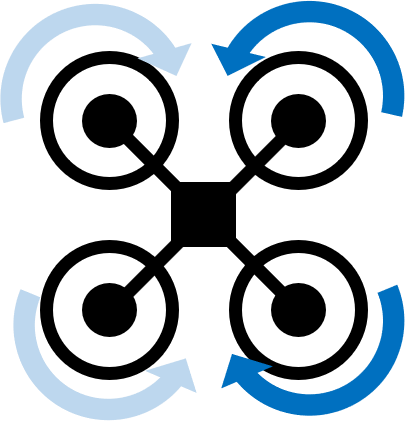
\includegraphics[scale=0.4]{img/drone_x_roll}
        \caption{Roll left}
        \label{fig:x-roll}
    \end{subfigure}
    ~
    \begin{subfigure}[b]{0.3\textwidth}
        \centering
        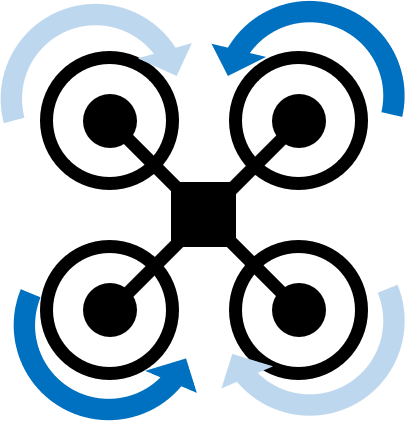
\includegraphics[scale=0.4]{img/drone_x_yaw}
        \caption{Yaw left}
        \label{fig:x-yaw}
    \end{subfigure}
    
    \caption{Using differential thrust to obtain 6-DOF movement. }
    \label{fig:rpas_6dof}
\end{figure}

\textbf{Hexacopter X:}
The hexacopter has all the stability benefits of a quadcopter as well as extra redundancy. The MRPAS could still land safely even if it experienced up to two simultaneous motor failures. Since the hexacopter uses two more motors than the quadcopter configuration, naturally, the RPAS of this configuration is generally bigger and can lift more payload. Of course, with the added components, it is also much more expensive to build, operate, and maintain. Furthermore, hexacopter RPAS's extended size and mass can cause more damage upon a crash.

We choose to the quadcopter configuration. 
The payload is not too heavy -- our target maximum payload weight is less than 500 g (\textbf{NF.DR.1}). The quadcopter configuration is also the most balanced in terms of the trade-off between cost and reliability. 

\subsubsection{Air Frame}\label{section:air-frame}

RPAS air frame sizes are commonly refered by their \textit{motor-to-motor-diagonal-span} (MMDS). The MMDS measures from a pair of motors that are the most far apart. 

The most common frame available for sale comes in 450 mm MMDS variants. 350 mm frames are also common amongst consumer products like the DJI Phantom series\cite{dji-phantom-3-specs} as seen in Figure~\ref{fig:djiphantom}. The frame size of 350 mm will constrain our ability to mount larger hardware --- posing a signifcant risk to integrating computing platform hardware. Additionally The 350 mm size also limits the propeller maximum size. The largest quadcopter configuration has an MMDS of 650 mm to 1000 mm and allow for extremely large payload capacity such as the one shown in Figure~\ref{fig:djis1000}. However, these are more commonly used for industrial or military applications.

\begin{figure}[h]
    \centering
    \begin{subfigure}[b]{0.33\textwidth}
        \centering
        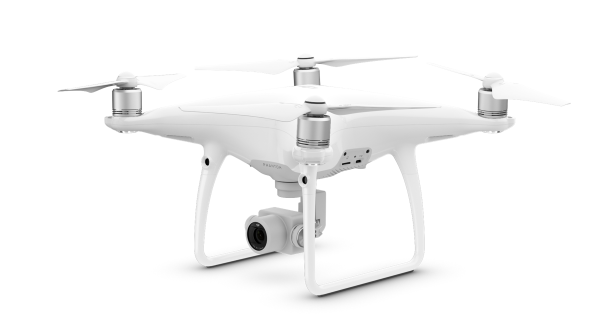
\includegraphics[width=\textwidth]{img/djiphantom4}
        \caption{DJI Phantom 4 (350 mm)}
        \label{fig:djiphantom}
    \end{subfigure}
    ~
    \begin{subfigure}[b]{0.33\textwidth}
        \centering
        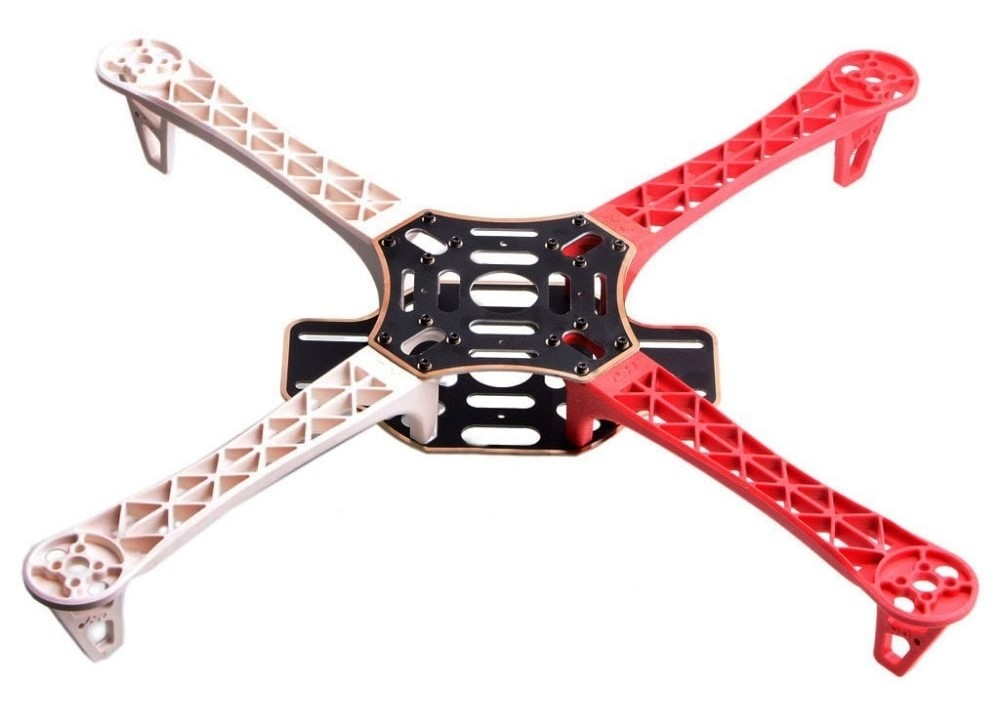
\includegraphics[width=\textwidth]{img/f450frame}
        \caption{Generic DIY frame kit (450 mm)}
    \end{subfigure}
    ~
    \begin{subfigure}[b]{0.33\textwidth}
        \centering
        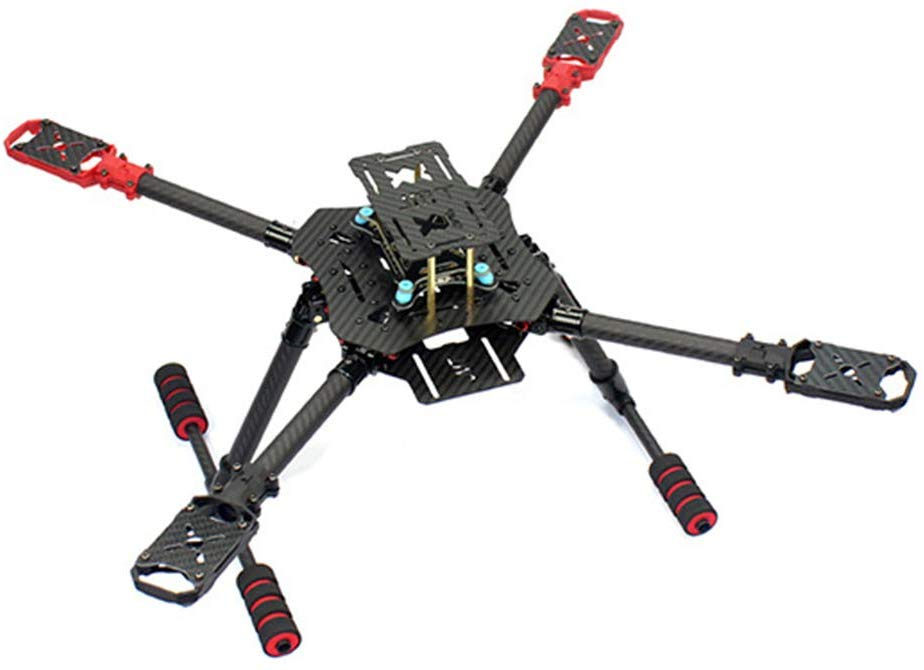
\includegraphics[width=\textwidth]{img/jmt560}
        \caption{JMT X4 Carbon Fiber Frame (560 mm)}
        \label{fig:jmtx4}
    \end{subfigure}
    ~
    \begin{subfigure}[b]{0.33\textwidth}
        \centering
        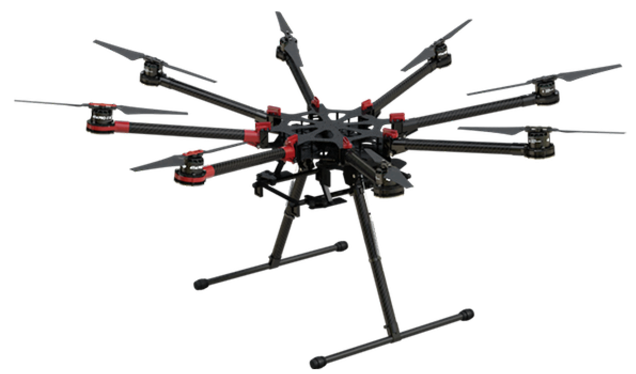
\includegraphics[width=\textwidth]{img/djis1000}
        \caption{DJI Spreadwings S1000 (1000 mm)}
        \label{fig:djis1000}
    \end{subfigure}
    
    \caption{Air Frame Options with Various Size Tiers }
\end{figure}

Our ideal option is a X4 560 mm MMDS carbon fibre frame from JMT, as shown in Figure~\ref{fig:jmtx4}. The frame is carbon fiber to enhance structural rigidity while keeping the system extremely lightweight. While the frame also features foldable arms and landing gear for portability, we consider replacing the hinges with static parts to reduce dead weight in order to achieve a longer flight time, as part of our non-functional requirements (\textbf{NF.DR.7}). The X4 560 mm frame is also wide enough to support propollers up to 14 inches in diameter. See Section~\ref{section:propsys} for reasons why a larger propeller is generally better.

For our testing rig (which is also our back-up drone), we are using the \textit{Flamewheel F450} frame with 450 mm MMDS. This design has many clones and variants and thus extremely cheap to purchase and replace on the internet. The frame has a adequate balance between portability and capability. However, the 450 mm frames can only support at most 12 inch propellers.

\subsubsection{Propulsion System}\label{section:propsys}

The propulsion system covers the majority of the RPAS parts list and determines the flight performance of the RPAS. 

\paragraph{Motor Type}

\underline{\textit{Brushed or brushless?}}
The MRPAS is electrically powered by a DC battery and we have two options for motors: DC brushed motors and DC brushless motors. Brushed motors use mechanical brushes in contact with the rotor’s commutator to switch polarity to sustain a constant rotation, whereas the brushless motors use electronic controllers to switch the polarity in the rotor. 

For flight applications, we chose the brushless DC (BLDC) motors for their extended usable lifetime. BLDC motors are also much more efficient than brushed motors because as they do not mechanically swap the polarity in the motor, which results in excess friction, heat, and potential sparking. 

\underline{\textit{Inrunner or outrunners?}}
BLDC motors are further broken down into two types: \textit{inrunner} and \textit{outrunner}. Inrunner motors have the rotor on the inside and the outrunner motors have the rotor on the outside.  As a result, the inrunners spins with a relatively lightweight rotor, which means inrunner motors typically spin fast but have low torque (i.e. inrunner motors have high KV constants; see Appendix~\ref{appendix:droneengine} for KV relationships). In order to obtain useful torque from the motor, we need to design and install a separate gearbox to convert the mechanical energies\cite{invsoutrunner}. The outrunner has a more massive rotor and so the spin-up time due to the additional inertia, but we can consider this as a benefit: the rotating mass is further from the center of rotation, thus the angular momentum helps to stabilize the rotor and reduce vibrations --- which is a major loss of efficiency. For an MRPAS typically mainly operating in stabilized flight and hover, this ``compromise'' is acceptable. Lastly, outrunners technologies are more modern and more serviceable than inrunner motors\cite{invsoutrunner}. For the reasons above, we choose outrunner motors.

\paragraph{Motor Size and Speed}\label{section:motor-speed}

Commercial outrunner BLDC motors generally have the following design parameters: rotor size, KV or KT constants, voltage, maximum rated power, and weight. Please refer to Appendix~\ref{appendix:droneengine} for the relationship between the aforementioned design parameters. Our design process consists of screening and ranking the best motors using the following order:

\begin{enumerate}
    \item Voltage: we choose motor that operates between 12.0 V to 20.0 V which is enough for heavy operations.
    \item KV constant: Since the motors' RPM-per-volt ratio (KV constant) is inversely proportional of torque-per-current ratio (KT constant), manufacturers typically only focus on the KV constant. We choose motors that has KV constants between 500 KV to 1000 KV. These constants are considered low-speed and high-torque characteristics and are typically used for large drones and endurance flights. We also choose this range so the propellers can spin slower and more efficiently, which extends the maximum flight time.
    \item Rotor size: As mentioned in the previous section regarding inrunners vs. outrunners, larger rotors implies a lower KV and higher KT. As a result, we choose the appropriate size based on the 500 KV to 1000 KV range. Markets show that sizes denoted 3508 to 2212 are adequate.
    \item Maximum rated power: KV and KT constands are simply linearized and simplified model for motor characteristics. The maximum power output is due to realistic non-idealities such as heat, motor resistance, and mechanical limits. Typically 500 KV to 1000 KV motors have a rating between 150 W to 400 W depending on the brand. We optimize for the most performant option allotted by our budget.
    \item Weight: Given the rotor size have been chosen, the weight of the motors have little variances, thus we prioritize this parameter the least and we optimize for the most compact or light option allotted by our budget.
\end{enumerate}

Using the above decision process, we determine that we are using T-Motor 3508 520 KV motor. For our testing rig, since it uses a smaller frame and a set of smaller propellers, we choose T-Motor Air Gear 350 (2213 920 KV) motors.

\paragraph{Propeller Material}

Common RPAS propellers are constructed using either plastic or carbon composite. Plastic is cheap, abundant, 
and relatively flexible. Due to their cheapness, however, their manufacturing is not as precise, leading to 
aerodynamic inefficiencies. Plastic propellers often require balancing where tape is applied to one of the 
blades such that the weight is balanced---minimizing vibrations. Carbon composite propellers, such as 
carbon fibre blades, are extremely light and subsequently much more expensive. The carbon composite 
propellers have micro-meter precision manufacturing, however, providing top efficiency. Carbon composite 
propellers are not flexible and extremely tough. It is more dangerous for persons to be near spinning 
carbon composite propellers due to their sharpness and toughness, and could lead to serious injuries or death.

For the final deliverable we choose carbon fiber propellers to maximize efficiency, flight time,and longevity for our client. But due to budget constraint and safety concerns, we chose plastic propellers for our testing rig.

\paragraph{Propeller Size and Pitch}

\textbf{Notation: } Propeller size and pitch is commonly denoted by RRYY where RR is the propeller diameter in inches, and YY is the propeller pitch in degrees. (9050 denotes a propeller with 9 inch diameter, and 5.0 inches of pitch; 1045 denotes a propeller with 10 inch diameter, and 4.5 inches of pitch).

\begin{figure}[h]
    \centering
    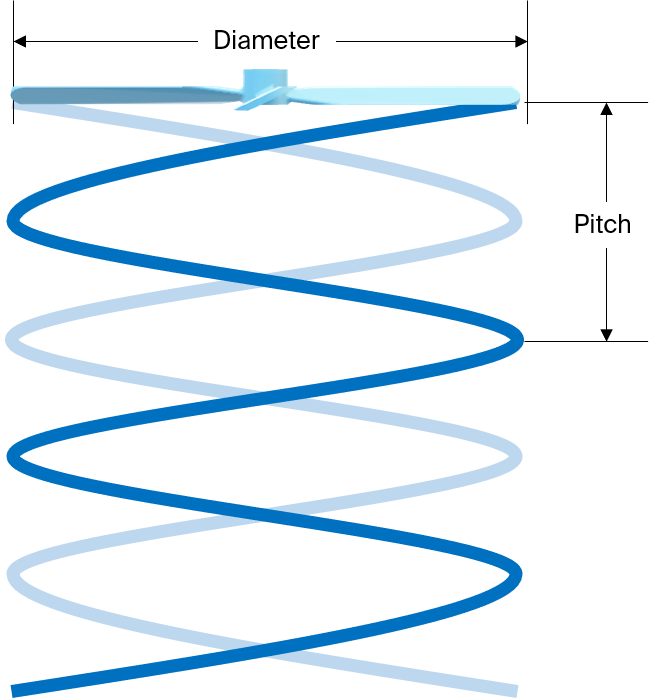
\includegraphics[scale=0.5]{img/proppitch}
    \caption{Propellor Diameter and Pitch Parameters}
    \label{fig:propeller}
\end{figure}

To obtain maximum thrust with low speed (low speed is more desirable, as mentioned in Section \ref{section:motor-speed}), we want to choose the biggest possible propeller diameter.

\begin{figure}[h]
    \centering
    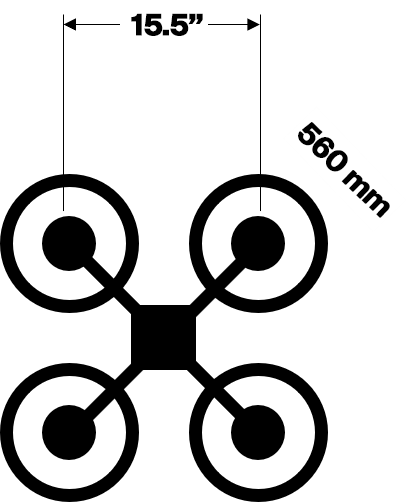
\includegraphics[scale=0.5]{img/framepropsize}
    \caption{Maximum Propeller Sizes}
    \label{fig:framepropsize}
\end{figure}

As mentioned in Section \ref{section:air-frame}, we chose the 450 mm frames, which means that the motor to motor 
adjacent span (MMAS) is about 12.5 inches. It is safe to provide 1 inch of clearance between propellers, 
therefore the ideal size of propellers to choose is 10 or 11 inches.

Mentioned in Section \ref{section:motor-speed}, we chose low-speed motors for their efficiency. And recall that 
given the same power: a slow-speed motor provides inversely proportional torque, so we chose propellers 
with relatively high pitch (between 3 to 5 inches) to take advantage of the high-torque output and to
maximize thrust output.

For the deliverable drone, we are using carbon fiber propellers with sizes 1145, 1245, or 1445. For our testing rig, the accetable sizes are: 1030, 1045, 1130, and 1145.

\paragraph{Speed Controllers}

The electronic speed controller (ESC) controls the voltage, current, and phase supplied to a BLDC motor. Since BLDC motors function by rotating magnetic field using electric commutation, the ESCs need to precisely control the timing and phase of the input to the three phase lines. All ESCs function similarly and the design parameters are size/weight, power rating, power efficiency, and cost.

As shown in Table 2, the typical maximum current draw is approximately 30 A. For a 
safety margin of 10 A, we decided to select ESCs with maximum rating of 40 A. All of the following options are appealing:

\begin{table}[h]
    \centering
    \caption{ESC Purchasing Options}
    \label{table:esc-table}

    \begin{tabular}{lrrrll}

    \hline
    \textbf{ESC} & \textbf{Rating} & \textbf{Weight} & \textbf{Price}  & & \textbf{Vendor}\\
    & [A] & [g] & [CA\$] & & \\
    \hline
    HAKRC BLHeli Dshot1200 & 35 & 7  & 40.00 & per 4 & Banggood\\
    Racestart RS30A Lite & 30 & 6  & 40.00 & per 4 & Banggood\\
    Racestart SPROG X DShot600 & 35 & 4  & 30.00 & per 4 & Banggood\\
    Skystars Talon32 & 40 & 7  & 12.00 & per 1 & Banggood\\
    \hline

    \end{tabular} 
\end{table}

\subsubsection{Flight Controller Units}

Flight controllers units (FCU) or sometimes short as FC come in different tiers differentiated by their price and target application/market. 

The cheapest FCU typically only has the bare-minimum features for flight (such as accelerometers and self-hover functions). These flight controllers are typically designed for acrobatic or basic VLOS flying and typically cost CA\$20 to CA\$50. The firmware that runs on these FCUs are typically open-source but nonetheless user-friendly and easily-programmable. Below is a list of FCs which falls under this tier:

\begin{itemize}[noitemsep,topsep=0pt, parsep=4pt, partopsep=0pt]
    \item F1, F3, F4, F7 FC are minimal in weight and footprint; they are ideal for light-weight operations.\cite{f1fc}
    \item KK 2.15 FC features a built-in display on the board, allowing quick access to flight settings without the need to connect to a computer for reprogramming.
    \item Naze32 FC is reliable with auto-tuning PIDs.
    \item CC3D FC is reliable with auto-tuning PIDs.
\end{itemize}

The next tier of FCs have more advanced features such as GPS-hold, autonomous flight, anto-land, telemetry, etc. They are designed for more advanced operation. These FCs are more expensive, costing CA\$50 to CA\$200, however these FCs have excellent after-sale support for their respective 
manufacturers and their documentation is better. Along 
with frequent manufacturer firmware updates, the mid-tier FCs are more reliable. The downside is that 
they are typically heavier and take up a much larger footprint. 
Below is a list of mid-tier FCs:

\begin{itemize}[noitemsep,topsep=0pt, parsep=4pt, partopsep=0pt]
    \item ArduPilot APM 2.8 is a flight controller using Arduino Mega and supports GPS and telemetry.
    \item Pixhawk PX4 Autopilot features pre-programmable autonomous operations.
    \item DJI Naza M Lite.
\end{itemize}

For the applications we require, we chose the ArduPilot APM 2.8 or the Pixhawk PX 4 as it is the most flexible option with advanced features at a reasonable price of CA\$75.00. Additionally, due to of the low-cost of low-tier FCs, we will also purchase one of the Naze32 or CC3D FC modules as a back-up.

\subsubsection{Radio Systems}

The minimum number of channels required to fly a drone is 4 -- one for each control: throttle, yaw, 
pitch, and roll. For this reason, we opted for the cheapest radio transmitter (TX) and receiver  (RX) 
combo we found from online vendors. 
The FlySky-FS i6 2.4GHz 6-Channel TX and RX bundle is ideal for our application due to its low cost.
According to the FlySky-FS i6 datasheet\cite{flyskyi6}, the radio frequency (RF) peak power is below 20 dBm while still achieving a maximum control range of 500 m (\textbf{NF.DR.4}).

\subsubsection{Battery}

We chose lithium polymer (Li-Po) batteries as they have the highest energy density (highest capacity to weight ratio) similar to that of lithium-ion (Li-ion) batteries, and thus are perfect for high-power, low-weight applications. Figure~\ref{fig:batterytypes} shows a graph of energy density of types of batteries \cite{battery} --- from this graph, it is clear that Li-Po batteries are to be chosen.

\begin{figure}[h]
    \centering
    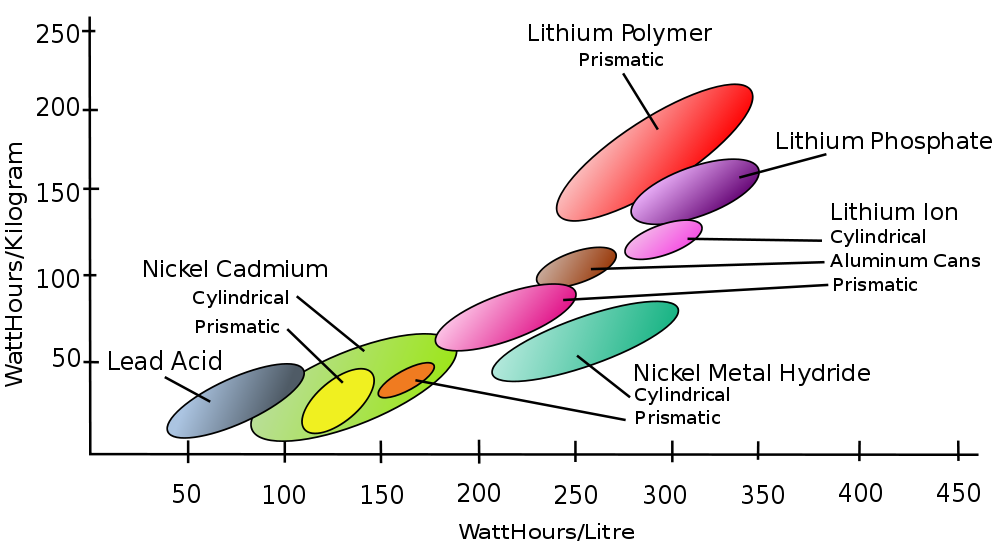
\includegraphics[width=0.5\textwidth]{img/energydensity.png}
    \caption{Energy Density Graph of Various Battery Types}
    \label{fig:batterytypes}
\end{figure}

Li-Po batteries have mainly three design parameters: configuration, capacity,  discharge rating, and internal resistance.

\textit{Configuration} is how the Li-Po batteries are manufactured and wired together: a single cell in a Li-Po battery provide a 
nominal voltage of 3.7 V due to its electrochemistry.
Similar to how portable electronics and appliances require AA or AAA batteries placed in a certain order, a single cell of 3.7 V is not enough to drive anything powerful. Ergo multiple cells can be wired in series and the 
voltage adds up: 2 cells in series, denoted as``2S'' batteries, have 7.4 V output, 3S batteries have 11.1 V output, and 4S batteries have a 14.8 V output. 

Battery \textit{capacity} is measured in watt-hours (Wh) or milli-amp-hours (mAh), which are units of electric power multiplied by units of time. A 20.0 Wh battery can output 20.0 W for 1.0 hour. Multiple battery cells can be put in parallel and their capacity adds up. A pair of four-cell batteries wired in parallel, denoted by ``4S2P'' has a 14.8 V output while having double the capacity of a single 4S battery of the same variant.

The \textit{discharge rating} is denoted by ``C'' and indicates the ratio of the capacity and the maximum discharge current which can be  safely discharged without significantly harming the battery's life. A 1,000 mAh battery with a discharge rating of 20 C can discharge a maximum of 1.0 A $\times$ 20 C = 20 A. It is important to note that a high discharge rating does not imply improved performance due to its \textit{internal resistance}. A higher internal resistance implies that the battery can run less efficiently, as power is lost internally\cite{battery-c}. We will thus choose the battery with the most optimal internal resistance as allotted by our budget. 

We will choose the design parameters for the battery after we have consolidated on the rest of the parts for the RPAS -- allowing for more system flexibility. 
